\subsubsection*{Pulsaciones}


\vspace{-1cm}
\item \label{pendacop}
\begin{minipage}[t][2.2cm]{0.75\textwidth}
Anteriormente se pidió obtener frecuencias y sus modos normales de oscilación de este sistema con dos péndulos de igual longitud $l$ pero de masas diferentes $m_{a}$ y $m_{b}$, acoplados mediante un resorte de constante $k$.
\end{minipage}
\begin{minipage}[c][3cm][t]{0.2\textwidth}
%   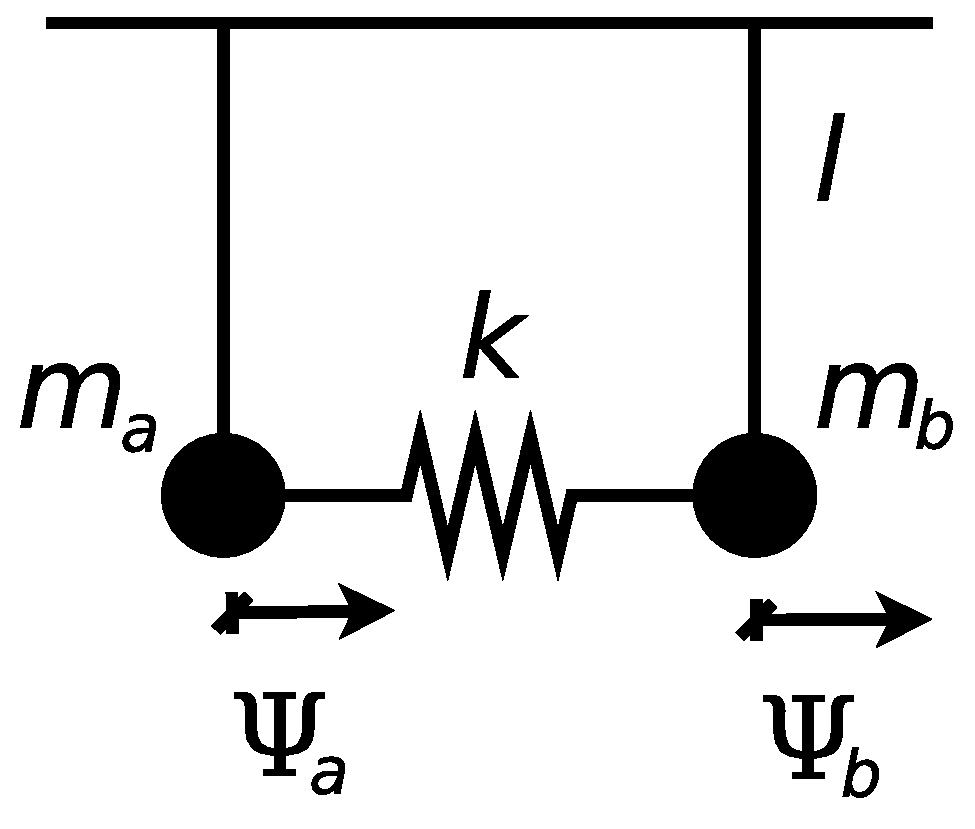
\includegraphics[width=\textwidth]{ej1-7}
	\begingroup
		\tikzset{every picture/.style={scale=0.4}}%
		\begin{tikzpicture}


\coordinate (A) at (-2.5,0);
\coordinate (B) at (2.5,0);

\draw[thick](-2.5,6)--(A);
\draw[thick](2.5,6) --(B);
% \draw[snake=zigzag,thick](A)--node[anchor=south]{\large {$k$}}(B);
\draw[decoration={aspect=0.7, segment length=5, amplitude=3, coil},decorate](A) -- node[anchor=south]{$k$}(B);

\draw[-LaTeX,thick](-4,4)--node[anchor=west]{\Large $\vec{g}$}(-4,2);

\dimline[extension start length=-0.25, extension end length=-0.25]{(-2.5,-1.3)}{(2.5,-1.3)}{\(\ell_0\)}; % cota resorte izq 2 

\dimline[extension start length=-0.25, extension end length=-0.25]{(3.5,0)}{(3.5,6)}{\(l\)};

\fill (A) node {\color{white} $m_a$} circle(0.7);
\fill (B) node {\color{white} $m_b$} circle(0.7);

\draw[-LaTeX,thick](-2.5,-3) --node[anchor=south]{$\Psi_a$}(-1,-3);
\draw[-LaTeX,thick](2.5,-3) --node[anchor=south]{$\Psi_b$}(4,-3);

% \draw[very thick](-3,6)--(3,6); % techo
\draw [very thick] (-3,6) coordinate (screen) -- (3,6); % pared superior
\fill [pattern = north east lines] (screen) rectangle +(6,0.5); % pared superior pattern


\end{tikzpicture}
}
	\endgroup
\end{minipage}
\begin{enumerate}
	\item Suponga que el acoplamiento es débil ($k\ll\frac{g}{l}\frac{m_{a}m_{b}}{m_{a}+m_{b}}$) y que las condiciones iniciales son: $\dot{\Psi}_{a}(0)=0,\dot{\Psi}_{b}(0)=0,\Psi_{a}(0)=0,\Psi_{b}(0)=1$.
Obtenga el movimiento de cada masa y grafíquelo en función del tiempo.
	\item Calcule los valores medios, en un ciclo rápido, de $T_{a}$ y $T_{b}$, donde $T$ indica energía cinética.
	Grafique $\left\langle T_{a}\right\rangle $ y $\left\langle T_{b}\right\rangle $, y analice las diferencias en el gráfico como función de las diferencias entre las masas ($m_{a}=m_{b}$ y $m_{a}$ muy diferente de $m_{b}$).
	Calcule el valor medio de la energía de interacción entre las dos partículas.
\end{enumerate}



\item \label{2masitas}
\begin{minipage}[t][1.5cm]{0.7\textwidth}
Anteriormente se pidió obtener frecuencias y los modos transversales del sistema de la figura.
Las masas están apoyadas en una mesa sin rozamiento, sujetas a las paredes por resortes de constante $k$ y unidas por otro resorte de constante $k'$.

¿Bajo qué condiciones espera observar batidos?
¿Qué son los batidos?
\end{minipage}
\begin{minipage}[c][0cm][t]{0.25\textwidth}
  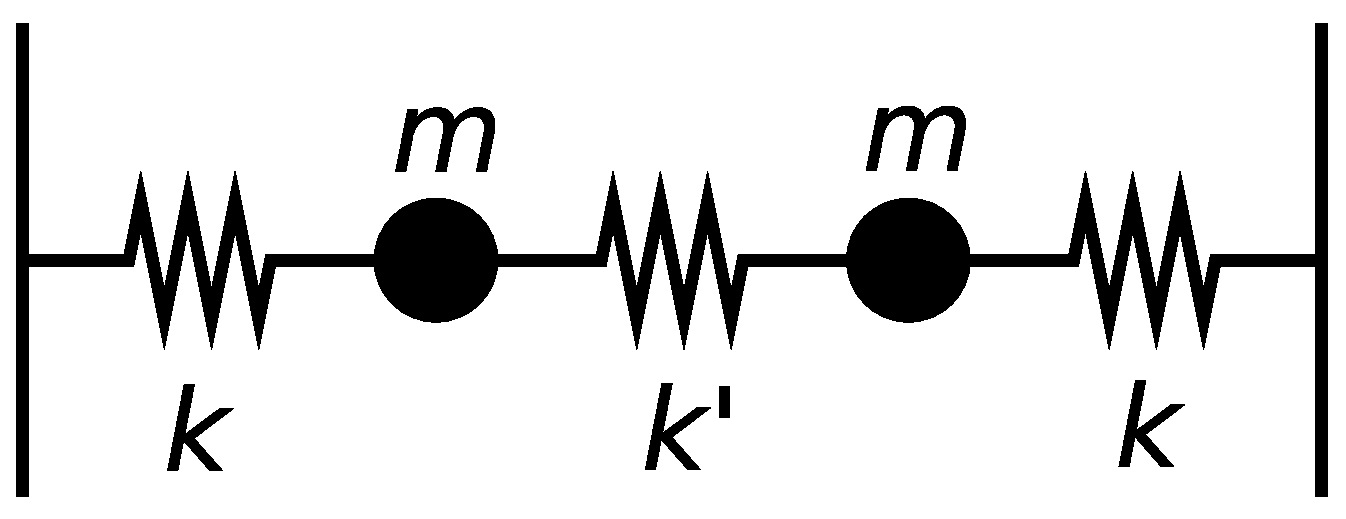
\includegraphics[width=\textwidth]{ej1-8}
\end{minipage}
